\section{量子カオスとしてのSYK模型\label{sec:syk_as_quantum_chaos}}

\subsection{量子重力の揺らぎ}
量子重力の大きい謎の1つは, ブラックホールのミクロな状態が持つ離散スペクトラムの起源である. 
量子論が本質的に持つ離散スペクトラムの存在は, 2点関数を用いる事によって調べる事ができる:
\begin{align}
	G(t)
		&= \frac{1}{Z(\beta)}\mathrm{tr}\left[e^{-\beta H}O(t)O(0)\right]\nonumber\\
		&= \frac{1}{Z(\beta)}\sum_{m, n}e^{-\beta E_m}
			|\langle m|O|n \rangle|^2e^{i(E_m - E_n)t}.
	\label{eq:twopointfunc_of_O}
\end{align}
ここで$O$はあるエルミート演算子, $Z = \mathrm{tr}(e^{-\beta H})$は分配関数, 
そして$|n\rangle$は固有値$E_n$を持つエネルギーの固有状態である. 
$t$が小さい時は級数を粗子化して滑らかな密度の積分に置き換える事ができ, $G(t)$は指数関数的にゼロに減少する. 
しかしこの振る舞いはずっと続く訳ではなく, $t$が大きい時にはスペクトラムの離散性が重要になっていき, 
\eqref{eq:twopointfunc_of_O}式の波の位相によって$G(t)$は激しく振動し, もはやゼロには落ちない. 

ホログラフィック原理において, 粗子化による近似は古典重力への量子補正を加えた摂動計算と同じであり, 
この近似の範疇では$G(t)$の値はずっとゼロに向かって減少し続ける. 
よって量子論の持つ離散性が見えておらず, 量子重力ではそれに対する補正項の存在があるはずである. 

離散スペクトラムの存在を調べるには, 2点関数よりも次式のような量を用いる方が単純化される:
\begin{align}
	Z(\beta, t) = \mathrm{tr}\ e^{-\beta H - itH}.
\end{align}
これは分配関数$Z(\beta)$を$\beta\to\beta + it$のように解析接続して得られる. 
$t$が大きい時では$Z(\beta, t)$は$G(t)$と同様に激しく振動する. 

$t$が大きい時のある量の振る舞いを調べるには時間平均を取るという事がしばしば行われる. 
$Z(\beta, t)$の時間平均はゼロであるので, $Z(\beta, t)$は大きい$t$でゼロのまわりで揺らぐという事が言える. 
その揺らぎの大体のサイズは
\begin{align}
	\left|\frac{Z(\beta, t)}{Z(\beta)}\right|^2
	= \frac{1}{Z(\beta)^2}\sum_{m,n}e^{-\beta(E_m + E_n)}e^{i(E_m - E_n)t}
\end{align}
で与えられる. 
一般にこの揺らぎのサイズの$t \gg 1$での振る舞いを調べるのは容易ではないが, 
長時間平均を取る事によって計算がいくらか簡単になる. 
長時間平均を取ると有限の位相を持つ波は全てゼロに均され, $E_n-E_m = 0$の項のみが残り, 次式にたどり着く:
\begin{align}
	\lim_{T\to\infty}\frac{1}{T}\int_0^Tdt\ \left|\frac{Z(\beta, t)}{Z(\beta)}\right|^2
	= \frac{1}{Z(\beta)^2}\sum_E N_E^2e^{-2\beta E}.
\end{align}
ここで$N_E$は縮退度であり, スペクトラムに縮退が存在しない ($N_E = 1$)ならば
\begin{align}
	\lim_{T\to\infty}\frac{1}{T}\int_0^Tdt\ \left|\frac{Z(\beta, t)}{Z(\beta)}\right|^2
	= \frac{Z(2\beta)}{Z(\beta)^2}
	\label{eq:average_of_fluctuation_of_Z}
\end{align} 
となる. 
$Z$のスケールは一般的にエントロピー$S$とある定数$a > 0$を用いて$Z \approx e^{aS}$である. 
よって$Z$の揺らぎの長時間平均\eqref{eq:average_of_fluctuation_of_Z}式は大体
$e^{-aS}$という大きさを持つ. 
AdS/CFT対応の文脈では$S$はブラックホールエントロピーであり, そのスケールは, 
バルク理論のストリング結合定数$g_s$とニュートン定数$G_N$を用いて, $1/g_s^2 \approx 1/G_N$で与えられる. 
よって\eqref{eq:average_of_fluctuation_of_Z}式はバルク理論における非摂動計算となる. 
ラージブラックホールでは$S$は境界側の場の理論の熱力学的エントロピーであり, その大きさは系の自由度で
与えられる. 
超対称性非可換ゲージ理論ならば$S\approx N^2$であり, SYK模型ならば$S\approx N$となる. 
いずれにせよ\eqref{eq:average_of_fluctuation_of_Z}式は$1/N$の非摂動的量である. 

ここで\eqref{eq:average_of_fluctuation_of_Z}式の左辺を粗子化近似によって計算しようとすると, 
離散スペクトラムを走る和が滑らかな密度の積分に置き換わり, 結果としてゼロとなり
\eqref{eq:average_of_fluctuation_of_Z}式の右辺と一致しない. 
よって$Z$の揺らぎの大きさがゼロにならないのは何故かを探求する事で, 
ブラックホールのスペクトラムの離散性や量子論を探る事ができる. 
この研究において, $\mathcal{N}=4$超対称非可換ゲージ理論よりも解析が可能という理由で
SYK模型は良い``実験室"となっている. 

以下では, 基本的にはSYK模型における分配関数の揺らぎの大きさの平均を調べる事になる. 
ただしSYK模型はランダム結合定数$J_{ijkl}$を持つので, 長時間平均の代わりに$J_{ijkl}$で平均を
取る(disorder average):
\begin{align}
	g(\beta, t) \equiv
	\frac{\average{Z(\beta, t)Z(\beta, t)^*}_J}{\average{Z(\beta)^2}_J}.
	\label{eq:spectral_form_factor}
\end{align}
ここで分母と分子をまとめて平均操作を施すという選択肢もあるが, ここでは別々に分子と分母の平均を取った. 
このような量を annealed quantity という. 
こうするメリットとしてはレプリカの数が有限で済むという事が挙げられる. 
すなわち, \eqref{eq:spectral_form_factor}式は基本的に$ZZ^*$の期待値なので, 
言ってみれば$Z$に対応する系と$Z^*$のそれというようにSYKの系を2つコピーしたと言える. 
もし分母と分子をまとめて平均取ったとすると, このコピーの数が任意個になってしまう. 

$g(t)$は量子カオスの分野において重要なスペクトラル統計の量であり, 
スペクトラル形状因子と呼ばれる. 
スペクトラル統計ではランダム行列理論(Random Matrix Theory: RMT)という数学が用いられる. 
量子カオスの分野における基本的な仮定の1つに, エネルギー固有値の統計的構造がRMT
におけるランダム行列のそれと一致するというものがある. 
このランダム行列の要素が従う確率分布には3種類あり, それぞれGaussian Unitary Ensemble(GUE),
Gaussian Orthogonal Ensemble(GOE), Gaussian Symplectic Ensemble(GSE)と呼ばれる. 
どれを用いるかは系の持つ対称性によって決まる. 
RMTは基本的に複数の固有値の相関の情報を持つ量の計算に使われる. 
特に$g(t)$はある程度値の離れた2つの固有値についての相関に関する情報を持つ. 
後にSYK模型のスペクトラル形状因子の$t \gg 1$における振る舞いはRMTによって説明される事を見る. 

\subsection{スペクトラル形状因子}
スペクトラル形状因子\eqref{eq:spectral_form_factor}式は, 数値解析によって
SYKハミルトニアンを対角化し, その固有値を集め, これを複数回施行してdisorder averageを取ると
グラフにプロットする事ができる(図\ref{fig:spectralformfactor}). 
$g(t)$の値は最初は落ちていくが, ある時刻からは上昇し始める. 
その後に長時間平均を与えるplateauに乗る. 
この節の目標のひとつはこの振る舞いの起源や, 示唆する所を理解する事である. 
\begin{figure}[ht]
	\centering
	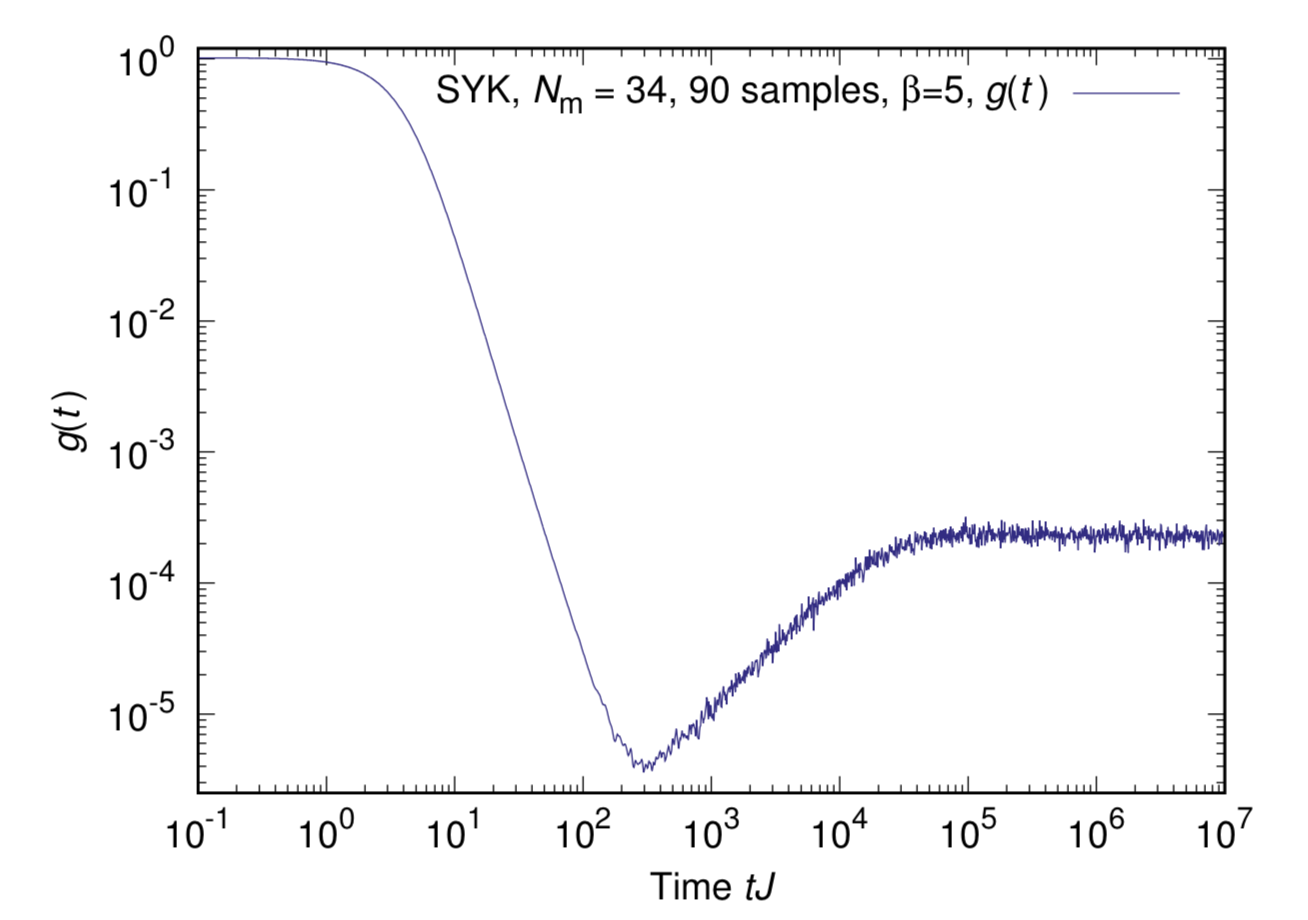
\includegraphics[width=10cm]{figures/spectralformfactor}
	\caption{SYK模型のスペクトラル形状因子. 粒子数は34個であり, 逆温度を$\beta = 5$としている. 
		また$J_{ijkl}$のサンプルを90個用意した. 
		ここでは横軸として時間に$J_{ijkl}$のスケール$J$を掛けて無次元化したものを用いた. 
		最初は$g(t)$の値がゼロに落ちている. この領域をslopeと呼ぶ. 
		その次には値が上昇している領域があり, この部分はrampと呼ぶ. 
		rampは$t$に比例している. 
		その後の水平な領域はplateauと呼ばれ, 長時間平均を取った際に現れる値である. 
		rampが終わってplateauに乗る時間をplateau時間$t_p$とする. 
		この図は\cite{polchinski_chaos}より引用した. 
	}
	\label{fig:spectralformfactor}
\end{figure}

$g(t)$はdisorder averageを取った量であり, ランダムカップリング$J_{ijkl}$についての揺らぎを
均したものであるため, 図\ref{fig:spectralformfactor}のplateauには量子論で期待される大きい揺らぎ
が存在しない
\footnote{小さい揺らぎは見られるが, 
	これは$J_{ijkl}$のサンプルを無限個にはできない事による数値計算上の理由である. }. 
disorder averageを取らず, 
1つの$J_{ijkl}$に対してのみプロットすると揺らぎが見られる\cite{polchinski_chaos}. 

$g(t)$は3つの領域に区分される. 
1つめは最初の値が降下している領域で, slopeと呼ばれる. 
2つ目は降下が終わって上昇する領域で, rampという. rampは$t$に比例している. 
ramp以降はplateauと呼ばれる領域が続く. plateauの高さが長時間平均である. 

SYK模型やRMTの$g(t)$には共にrampやplateauの構造が見られる. 
RMTにおける$g(t)$は具体的な解析が行われおり, 特に行列のサイズのラージ極限での議論をこの後に述べる. 
その後, それを踏まえてSYK模型に話を移す事にする. 

\subsubsection{ランダム行列理論のスペクトラル形状因子}
\begin{figure}[ht]
	\centering
	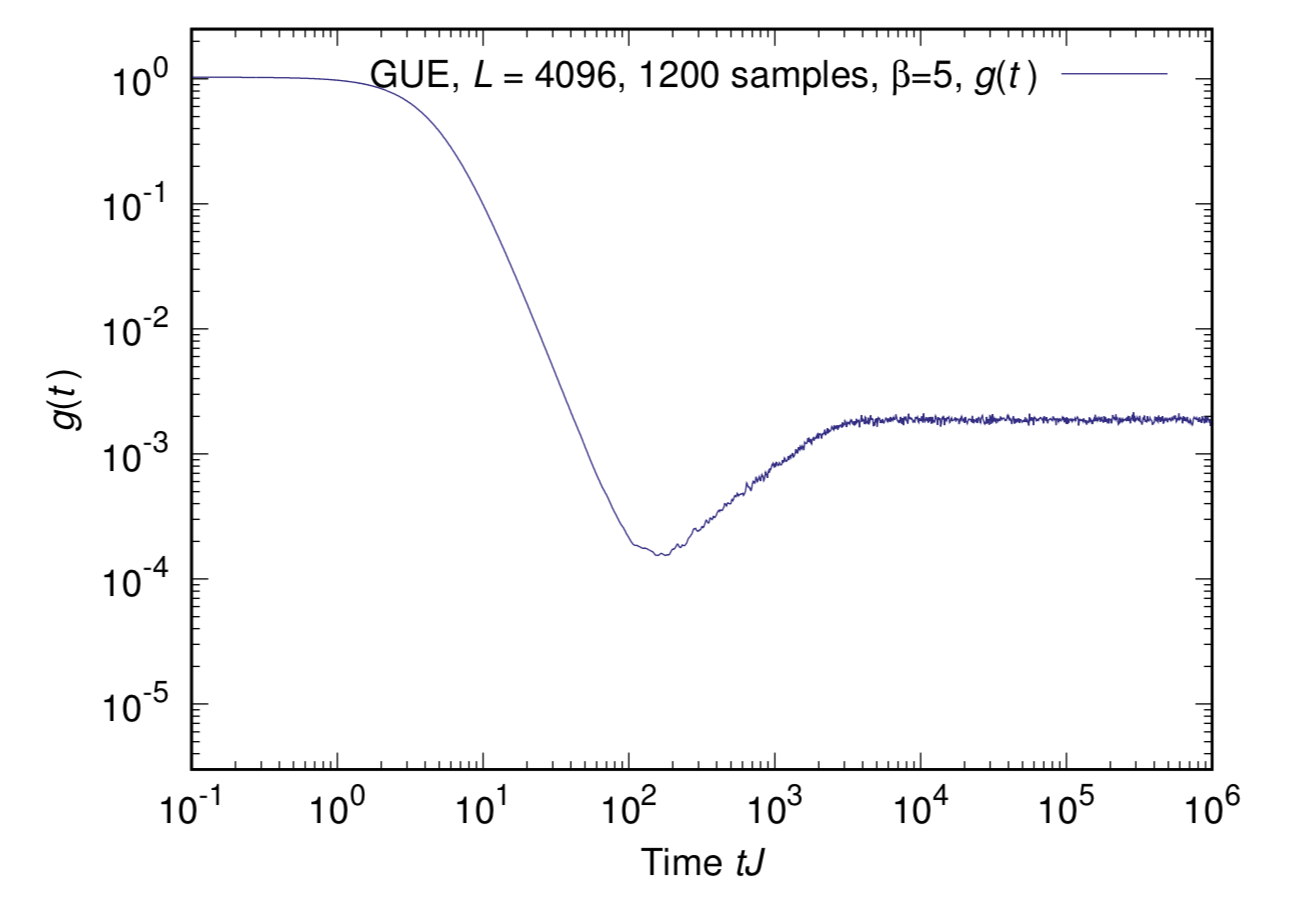
\includegraphics[width=10cm]{figures/spectralformfactor_inRMT}
	\caption{GUEにおけるスペクトラル形状因子. 逆温度は$\beta=5$, 行列のサイズは$L=4096$であり, 
		サンプル数は1200個である. この図は\cite{polchinski_chaos}より引用した. 
	}
	\label{fig:spectralformfactor_inRMT}
\end{figure}
ここではRMTの簡単なレビューを記述する. 
特にランダム行列の持つ乱数の従う統計集団としてGUEを選ぶ. 
この節の目標は図\ref{fig:spectralformfactor_inRMT}に表示されているGUEスペクトラル形状因子の, 
slopeのlate-timeでの振る舞いやrampの初期の振る舞いを理解する事である. 
結果は両方ともべき乗で表され, それを用いてslopeとrampが接続する時間を計算する. 
なお, この時間をdip timeと呼ぶ. 

階数$L$を持つエルミート行列$M$を考える. 
これがGUEに属するとすると, 統計平均は
\begin{align}
	\mathcal{Z}_{\mathrm{GUE}} = \int \prod_{i, j} dM_{ij}\ \exp\left(
		-\frac{L}{2}\tr\ M^2
	\right)
	\label{eq:GUEstatistics}
\end{align}
で与えられる. 
エルミート行列$M$はSYK模型でのハミルトニアンに相当し, 階数$L$はヒルベルト空間の次元に
対応する. 
RMTとSYK模型の間の重要な違いの1つは摂動パラメータの違いであり, SYK模型は$1/N$なのに対し, 
RMTは$1/L \approx e^{-N}$となっている.

$M$の分配関数は
\begin{align}
	Z(\beta, t) = \tr\ e^{-\beta M - iMt}
	\label{eq:GUEpartition_function}
\end{align}
で定義される. 
スペクトラル形状因子は\eqref{eq:spectral_form_factor}式と同様に定義される. 
ただしdisorder average $\langle \cdot\rangle_J$は\eqref{eq:GUEstatistics}式によるGUEの
統計平均$\langle\cdot\rangle_{\mathrm{GUE}}$に置き換わる. 

次にエルミート行列$M$を対角化し, 基底をユニタリ変換する事を考える. 
この変換により, 固有値同士の``排斥力"を表すヤコビアンが現れる. 
行列のサイズ$L$のラージ極限を取ると固有値分布はある密度$\rho$によって記述できる. 
この$\rho$を物理的な密度として使い, $\tilde{\rho}$を規格化したものとする:
\begin{align}
	\int d\lambda\ \rho(\lambda) = L,\hspace{20pt}
	\int d\lambda\ \tilde{\rho}(\lambda) = 1,\hspace{20pt}
	\rho(\lambda) = L\tilde{\rho}(\lambda).
\end{align}
\eqref{eq:GUEstatistics}式において$M$のスペクトルを$\tilde{\rho}$として滑らかにすると, 
GUEの統計平均は
\begin{align}
	\mathcal{Z}_{\mathrm{GUE}} = \int \mathcal{D}\tilde{\rho}(\lambda)\ e^{-S},
	\hspace{10pt}
	S 
	= -\frac{L^2}{2} \int d\lambda\ \tilde{\rho}(\lambda)\lambda^2
	+ L^2 \int d\lambda_1 d\lambda_2\ \tilde{\rho}(\lambda_1)\tilde{\rho}(\lambda_2)
		\log|\lambda_1 - \lambda_2|
	\label{eq:GUEstatistics_in_large_L}
\end{align}
と書き改められる. 
この$\mathcal{Z}_{\mathrm{GUE}}$のラージ$L$鞍点はウィグナー半円分布(Wigner semicircle law)
となる:
\begin{align}
	\average{\tilde{\rho}(\lambda)} = \tilde{\rho}_s(\lambda)\equiv
	\frac{1}{2\pi}\sqrt{4 - \lambda^2}.
	\label{eq:semicircle_law}
\end{align}
固有値間の間隔の平均値はおよそ$1/L$である. 

ここまでの準備を踏まえて, GUEのスペクトラル形状因子のslopeとrampについて議論する. 
直接$g$を計算しても良いが, dip time以前と以後で$g$に大きく寄与する成分を大雑把に
近似する事ができ, dip timeより前ならば非連結部分$g_d$, 後ならば連結部分$g_c$となる. 
$g_d$および$g_c$はそれぞれ次式で与えられる:
\begin{align}
	g_d(\beta, t)
	= \frac{\average{Z(\beta, t)}_{\mathrm{GUE}}\average{Z^*(\beta, t)}_{\mathrm{GUE}}}
		{\average{Z(\beta)}_{\mathrm{GUE}}^2},
	\label{eq:disconnected_piece}
\end{align}
\begin{align}
	g_c(\beta, t) = g(\beta, t) - g_d(\beta, t).
	\label{eq:connected_piece}
\end{align}
なおSYK模型においても$g_c$と$g_d$は同様にして与えられる(期待値計算はdisorder averageである). 

最初にdip time以前の振る舞いを調べる事にすると, 計算するべきは$g_d$である. 
簡単のため$\beta = 0$とする. 
分配関数のラージ$L$での振る舞いは半円分布によって与えられ, 次式のような結果となる:
\begin{align}
	\average{Z(\beta=0, t)}_{\mathrm{GUE}}
	= \int_{-2}^2 d\lambda\ L\tilde{\rho}_s(\lambda)e^{-i\lambda t)}
	= L\frac{J_1(2t)}{t}
	\approx \frac{L}{t^{3/2}}
	\hspace{10pt}(t \approx \mathrm{large}).
\end{align}
ここで$J_1$は第1種ベッセル関数である. 
よって$t \gg 1$において
\begin{align}
	g(\beta = 0, t) \approx g_d(\beta = 0, t) \approx \frac{1}{t^3}
	\label{eq:late_time_slope_in_RMT}
\end{align}
となる. 有限温度で計算しても計算結果は同じである. 

次にdip time以降の時間に移り, rampの存在を導く. 
この時$g \approx g_c$となり, 両方とも
rampやplateauを与えるため$g$と$g_c$のどちらを選んでも良いが, 
$g_c$のrampは初期時刻のあたりまで伸びているため摂動計算がやりやすい. 

$g_c$は
\begin{align}
	g_c(\beta = 0, t)
	= \int d\lambda_1 d\lambda_2\ 
		R_2(\lambda_1, \lambda_2)e^{i(\lambda_1 - \lambda_2)t},
	\label{eq:g_c_with_beta_0}
\end{align}
\begin{align}
	R_2(\lambda_1, \lambda_2)
	= \average{\delta\tilde{\rho}(\lambda_1)\delta\tilde{\rho}(\lambda_2)}_{\mathrm{GUE}}
	\label{eq:fourier_transfomed_g_c}
\end{align}
で与えられる. 
ここで$R_2$は$\tilde{\rho}$の連結2点関数であり, また
$\delta\tilde{\rho}(\lambda) = \tilde{\rho}(\lambda) - \tilde{\rho}_s(\lambda)$
は半円分布からなる固有値密度\eqref{eq:semicircle_law}式まわりの揺らぎである. 
半円分布のちょうど真ん中付近では, $R_2$は次式のような正弦核の2乗とデルタ関数の和で与えられる:
\begin{align}
	R_2(\lambda_1, \lambda_2)
	= -\frac{\sin^2(L(\lambda_1 - \lambda_2))}{(\pi L(\lambda_1 - \lambda_2))^2}
		+ \frac{\delta(\lambda_1 - \lambda_2)}{\pi L}.
	\label{eq:sine_kernel_in_R2}
\end{align}
これを\eqref{eq:g_c_with_beta_0}式に代入して積分を計算すると
\begin{align}
	g_c(0, t) \approx 
	\left\{
		\begin{matrix}
			t/(2\pi L^2) \hspace{20pt}t < 2L\\
			1/(\pi L)    \hspace{29pt}t \geq 2L
		\end{matrix}			
	\right.
\end{align}
となる. 
これによってrampとplateauの存在が見て取れる:
$t = 2L$まではrampであり, その後は一定値を取りplateauに乗っている. 
ただしrampを見るには\eqref{eq:sine_kernel_in_R2}式において正弦核の近似値を
用いたもので十分である. すなわりrampそのものは
\begin{align}
	R_2(\lambda_1, \lambda_2) \approx -\frac{1}{2(\pi L(\lambda_1 - \lambda_2))^2}
\end{align}
から与えられる. 
しかしplateauの存在は正弦核を近似せずそのまま扱う必要がある. 
この議論が示唆するのは, rampは$1/L^2$を摂動パラメータとする摂動論による効果であり, 
plateauはそうではないという事である. 

これによってSYK模型に応用する際に次のような事が言える:
SYK模型ではヒルベルト空間の次元は$L = 2^{N/2}$なので$1/L \approx e^{-aN}$となる. 
従ってRMTにおける摂動的な効果はSYK模型では非摂動的である. 
またRMTでの非摂動効果は$O(e^{-L})$の大きさであり, これはSYK模型では$O(\exp(-e^{aN}))$
という極めて小さい非摂動的効果となる. 

\subsubsection{SYK模型のスペクトラル形状因子}
ここではラージ$N$ SYK模型におけるスペクトラル形状因子のrampやplateauの導出を行う. 
基本的には$\average{Z(\beta + it)Z(\beta - it)}$の計算であり, 
SYK模型における期待値$\average{\cdot}$はdisorder average $\average{\cdot}_J$となるが, 
これをGUEのラージ$L$での期待値\eqref{eq:GUEstatistics_in_large_L}式に近似して計算を進める. 
rampとplateauは第\ref{sec:effective_theory}節で論じたシュワルツ理論から与えられる. 

最初に系がGUE統計に従うとした場合の一般論からrampやplateauがどのように現れるかを見る. 
その後議論をSYK模型へ適用する. 
$\average{ZZ^*}$は一般に
\begin{align}
	\average{Z(\beta + it)Z(\beta - it)}
	= \int d\lambda_1d\lambda_2\ \average{\rho(\lambda_1)\rho(\lambda_2)}
		e^{-2\beta E}e^{-ixt}
\end{align}
と書ける. ここで
\begin{align}
	x = \lambda_1 - \lambda_2,\hspace{20pt}
	E = \frac{\lambda_1 + \lambda_2}{2}
\end{align}
である. 
なおここでは密度$\rho$は規格化されていないのものであり, $\int d\lambda\ \rho = L$である. 

$t \gg 1$においては$x \ll 1$となるような領域のみが積分に寄与すると考え, かつこの領域では
$\average{\rho(\lambda_1)\rho(\lambda_2)}$はRMTの統計集団で近似できると仮定する. 
簡単のため, ここでは前節で扱ったGUE統計を採用すると
\begin{align}
	\average{\rho(\lambda_1)\rho(\lambda_2)}
	= \average{\rho(E)}\delta(x)
		+ \average{\rho(\lambda_1)}\average{\rho(\lambda_2)}
		\left(1 - 
			\frac{\sin^2(\pi\average{\rho(E)}x)}{(\pi\average{\rho(E)}x)^2}		
		\right)
\end{align}
となり, これを用いて$\average{ZZ^*}$を計算すると
\begin{align}
	\average{Z(\beta + it)Z(\beta - it)}
	= |\average{Z(\beta + it)}|^2 + \int dE\ e^{-2\beta E}
		\min\left(\frac{t}{2\pi}, \average{\rho(E)}\right)
	\label{eq:average_of_ZZ}
\end{align}
を得る. 

次に\eqref{eq:average_of_ZZ}式をラージ$N$ SYK模型に適用して議論する. 
最初に右辺の第1項$|\average{Z(\beta + it)}|^2$を計算する. 
ラージ$N$の鞍点を用いて数値的に$\average{Z(\beta + it)}$を評価できるが, 
大きい$\beta + it$においては鞍点周りの揺らぎも考慮しなければならない. 
この揺らぎは第\ref{sec:effective_theory}節で論じたシュワルツ理論で与えられる:
\begin{align}
	Z_{\mathrm{Sch}}(\beta)
	= \int \frac{\mathcal{D}t(u)}{SL(2, \mathbb{R})}\ 
		\exp\left[
			-\frac{\pi N\alpha_S}{\beta\mathcal{J}}\int_0^{2\pi}du\ 
			\left(\left(\frac{t''}{t'}\right)^2 - t'^2\right)		
		\right].
	\label{eq:Schwartzian_theory_as_fluctuation}
\end{align}
ここで指数関数の肩の作用は\eqref{eq:action_for_epsilon}式で
$\epsilon$を$t$に書き換え, さらに$t\to 2\pi t/\beta$としたものを用いた. 
また$\mathcal{D}t$の下に存在する$SL(2,\mathbb{R})$は, 測度がこの変換群で不変という事を表している. 
この分配関数の古典的な寄与や1ループの寄与は\cite{maldacena}によって計算されており, 
\begin{align}
	Z_{\mathrm{Sch}}^{\mathrm{1-loop}}(\beta)
	= \frac{\mathrm{numerical\ const}}{(\beta \mathcal{J})^{3/2}}
		\exp\left(\frac{2\pi^2N\alpha_S}{\beta\mathcal{J}}\right)
	\label{eq:one_loop_Schwartzian}
\end{align}
という結果がある. 
しかしながら$\beta + it\gg 1$の時は\eqref{eq:Schwartzian_theory_as_fluctuation}式の
作用積分の前の係数は小さくなり, $t(u)$は大きく揺らぐ. 
大雑把に言えばこれによって摂動計算が破綻し, $Z$の計算が難しいものとなっているが, 
実は適切な測度のもとで理論は1-ループ完全である事が(間接的に)示されている\cite{polchinski_chaos}. 
従って\eqref{eq:average_of_ZZ}式の第1項$|\average{Z(\beta + it)}|^2$はスペクトラル形状因子
に次のような寄与を与える:
\begin{align}
	\frac{|\average{Z(\beta + it)}|^2}{\average{Z(\beta)}^2}
	= \frac{\beta^3}{(\beta^2 + t^2)^{3/2}}\exp\left(
		-\frac{cNt^2}{\beta(\beta^2 + t^2)}	
	\right).
	\label{eq:slope_in_SYK}
\end{align}
ここで$c$は\eqref{eq:specific_heat}式で与えられる比熱である. 
上式の指数関数による時間依存性は$t\sim \sqrt{N}$以降で無視でき, 
左辺は$\sim t^{-3}$となりRMTでのdip time直前の
slopeの振る舞い\eqref{eq:late_time_slope_in_RMT}式と一致する. 

次に\eqref{eq:average_of_ZZ}式の第2項の積分を計算する. 
ホログラフィック極限$\beta \sim \mathrm{large}$ においてエントロピーは
$S(E) = NS_0 + \sqrt{2c(E-E_0)N}$となる事を用い, さらに\eqref{eq:average_of_ZZ}式の積分から
1-ループの寄与を無視すると, $g(t)$に対して次のようなrampとplateauを与える寄与を得る:
\begin{align}
	g_{\mathrm{ramp}}\approx\left\{
		\begin{array}{l}
			\frac{t}{2\pi}\exp\left(-2NS_0 - \frac{cN}{\beta}\right)
				\hspace{110pt}\frac{t}{2\pi} < e^{NS_0}\\
			\frac{t}{2\pi}\exp\left(-2NS_0 - \frac{cN}{\beta}
			- \frac{\beta}{cN}\log^2\left(\frac{t/(2\pi)}{e^{NS_0}}\right)\right)
				\hspace{20pt}e^{NS_0} < \frac{t}{2\pi} < \frac{t_p}{2\pi}\\
			\exp\left(-NS_0 - \frac{3cN}{4\beta}\right)
				\hspace{120pt}t_p < t
		\end{array}		
	\right. .
	\label{eq:SYK_ramp_and_plateau_contribution}
\end{align}
ここで$t_p = 2\pi e^{NS_0 + cN/(2\beta)} = 2\pi e^{S(\beta)}$である. 
この式と\eqref{eq:slope_in_SYK}式を連立させるとdip time $t_d \sim e^{NS_0/2}$を得る. 

\subsection{スペクトラル形状因子の$G$, $\Sigma$による記述}
次にここではスペクトラル形状因子のslope, rampを与える寄与のフェルミオンの2点関数$G$
および自己エネルギー$\Sigma$による記述を述べる
\footnote{plateauはここでは述べない. 詳しくは第\ref{sec:conclusion}節で述べるが, 現時点では
plateauを与える寄与はわかっていない. }. 
これによりSYK模型に対応するJackiw--Teitelboim重力理論における
スペクトラル形状因子の解析に対してある程度の方針を得る. 
実際に第\ref{sec:gravity}節では得た方針を元にしてslopeやrampの構造を与える時空の計量を考える. 

$g(\beta, t)$は基本的には分配関数
$Z = \int \mathcal{D}\tilde{G}\mathcal{D}\tilde{\Sigma}\ 
\exp(-NS[\tilde{G}, \tilde{\Sigma}])$から与えられるものであり, 
従って$g(\beta, t)$の振る舞いの起源を調べるという事は
この経路積分に寄与するような$G$と$\Sigma$の場としての配位を探るという事である. 

また$g(\beta, t)$そのものは$\average{Z(\beta + it)Z(\beta - it)}_J$の計算であり, 
従ってあたかも逆温度がそれぞれ$\beta + it$と$\beta - it$であるような2つのSYK模型の
コピーを用意したように見える. 
このコピーはレプリカと呼ばれており, レプリカの数が2つで済む事が\eqref{eq:spectral_form_factor}式
の$g(\beta, t)$の定義式でdisorder averageを分子分母別々に施すメリットである. 
この2つのレプリカをL系, R系と名付ける事にする. 

この節の方針は次の通りである. 
まず簡単のため$\beta=0$として$\average{Z(it)Z(-it)}_J$を計算し, 
2つのレプリカ系が従う作用を導き出し, 経路積分に寄与するような鞍点を探る. 
slopeを与える鞍点は自明な解から構成されるものであり, L系とR系に相関がない. 
一方でrampを与える鞍点は非自明な解から成り, L系とR系が互いに相関する. 
この解はL系とR系がそれぞれ独立に持っていた時間並進対称性を自発的に破るものであり, 
そのソフトモードによって解はラベリングされている. 
その結果$g(t)$の経路積分のうちrampを与える部分はソフトモードを走る積分となり, 
その積分範囲が$t$までという事から$g \propto t$となり, rampを構築する. 
その後は一般の$\beta$について議論を拡張するのだが, 素朴に計算を試みても鞍点を見つける事はできない. 
これは系を低エネルギーへ押し出すようなある種の圧力の存在によるものであり, 
この不安定さを安定させるために小正準集団スペクトラル形状因子$Y_{E,\Delta}(t)$というものを導入する. 
このスペクトラル形状因子の変形版を用いて鞍点を探る事によって$\beta = 0$の場合と同様にslope/ramp構造
を見る事ができる. 

なお, 以下では$G$や$\Sigma$の時間変数と, 分配関数$Z$の虚軸の時間変数を区別するために, 
分配関数の持つ時間変数を大文字の$T$として$Z(\beta, T)$などと表記し, 
$G$や$\Sigma$の持つ時間変数には小文字の$t$を割り当て$G(t)$などと表記する. 

\subsubsection{$\beta = 0$の場合}
最初に$\average{Z(iT)Z(-iT)}_J$を計算する. 
上述したように2つのレプリカが現れ, $G$や$\Sigma$はそれぞれレプリカの添字を持つようになり, 
$G_{ij}(t,t')$や$\Sigma_{ij}(t,t')\ (i,j \in \{L, R\})$のようになる. 
結果は次式の通りである:
\begin{align}
	\average{Z(iT)Z(-iT)}_J
	= \int \mathcal{D}G\mathcal{D}\Sigma\ e^{-NI[G, \Sigma]},
\end{align}
\begin{align}
	I[G, \Sigma]
	= -\frac{1}{2}\log \det\left(
			\delta_{ij}\frac{\partial}{\partial t} - \Sigma_{ij}
		\right) + \frac{1}{2}\int_0^T\int_0^T dtdt'\ \left(
			\Sigma_{ij}G_{ij} - \frac{J^2}{q}s_{ij}G_{ij}^q
		\right).
	\label{eq:action_for_the_two_replicas}
\end{align}
ここで$s_{LL} = s_{RR} = -1,\ s_{LR} = s_{RL} = (-1)^{q/2}$である. 

$G$と$\Sigma$は2つの時間変数を持つが, 簡単のため以下ではそれらの差の関数であると仮定する:
\begin{align}
	G_{ij}(t, t') = G_{ij}(t - t').
\end{align}
$G$と$\Sigma$は元々のSYK模型のマヨラナフェルミオンに由来する周期$T$の反周期性を持つ. 
従ってフーリエ変換は
\begin{align}
	G_{ij}(\omega_n) = \int_0^T dt\ e^{i\omega_nt}G_{ij}(t),
	\hspace{20pt}\omega_n = \frac{2\pi}{T}\left(n + \frac{1}{2}\right)
\end{align}
となる. 
シュウィンガー・ダイソン方程式は
\begin{align}
	\begin{pmatrix}
		G_{LL}(\omega_n) & G_{LR}(\omega_n)\\
		G_{RL}(\omega_n) & G_{RR}(\omega_n)
	\end{pmatrix}
	=
	\begin{pmatrix}
		-1/(i\omega_n + \Sigma_{LL}(\omega_n)) & -1/\Sigma_{LR}(\omega_n)\\
		-1/\Sigma_{RL}(\omega_n) & -1/(i\omega_n + \Sigma_{RR}(\omega_n))
	\end{pmatrix}
	\label{eq:replica_SDeq_1}
\end{align}
\begin{align}
	\Sigma_{ij}(t) = s_{ij}J^2G_{ij}^{q-1}(t)
	\label{eq:replica_SDeq_2}
\end{align}
で与えられる. 

$G_{LR} = \Sigma_{LR} = 0$とすると, L系とR系に相関がないような方程式となり, 
その解を用いて$\average{Z(iT)Z(-iT)}_J$を計算するとラージ$T$でゼロに値が落ちていき, 
slopeを構成する. 
次にrampを与える配位を探るために非自明な鞍点を見つける. 
まず, この非自明な鞍点というものがそもそも存在するという事に対して動機付けを行う. 

\begin{figure}[ht]
	\centering
	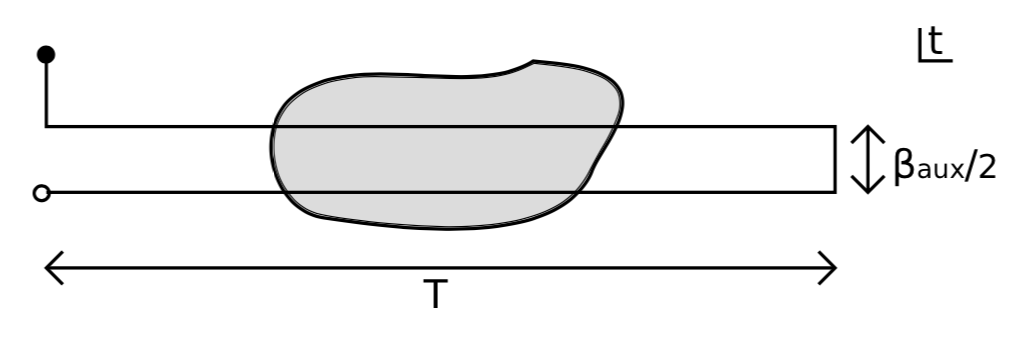
\includegraphics[width=10cm]{figures/beta_aux}
	\caption{$\tr(e^{-\frac{\beta_{\mathrm{aux}}}{2}H}e^{-iHT}e^{-\frac{\beta_{\mathrm{aux}}}{2}H}e^{iHT})$
		の経路積分による表示. 白い点と黒い点は同一のものである. 
		灰色の領域において$G$, $\Sigma$の鞍点方程式は元々の$Z(iT)Z(-iT)$でのそれに近いというのが
		基本的なアイディアである. この図は\cite{stanford_chaos}より引用した.
	}
	\label{fig:beta_aux}
\end{figure}
$Z(iT)Z(-iT)$の事は一旦忘れて
$\tr(e^{-\frac{\beta_{\mathrm{aux}}}{2}H}e^{-iHT}e^{-\frac{\beta_{\mathrm{aux}}}{2}H}e^{iHT})$
という量を考える. ここで$\beta_{\mathrm{aux}}$は任意のパラメータである. 
実時間での時間発展は互いに相殺し, $Z(\beta_{\mathrm{aux}})$となる. 
それでもこの量を図\ref{fig:beta_aux}のような4つの経路それぞれを計算する事はできる. 
この4つの経路の$G$, $\Sigma$の鞍点の配位は逆温度$\beta_{\mathrm{aux}}$の熱相関関数の解析接続である. 
基本的なアイディアは, 図\ref{fig:beta_aux}の横に長く伸びている経路の$G$, $\Sigma$の鞍点方程式は
元々の$Z(iT)Z(-iT)$でのそれと近似的に同じというものである. 

従ってシュウィンガー・ダイソン方程式\eqref{eq:replica_SDeq_1}式および
\eqref{eq:replica_SDeq_2}式の近似解として, 任意の逆温度$\beta_{\mathrm{aux}}$を持つ
解析接続された熱相関関数を使うと良い可能性がある. 
より正確には, 次式のように試験的な解としてL系とR系に対してThermofield Double State (TDS)にある
相関関数を用いるという事である:
\begin{align}
	G_{ij}^{\beta_{\mathrm{aux}}}(t)
	= \langle \mathrm{TDS}(\beta_{\mathrm{aux}})
		|\psi^i(t)\psi^j(0)|\mathrm{TDS}(\beta_{\mathrm{aux}}) \rangle,
	\hspace{20pt}i,j \in \{L, R\}.
\end{align}
しかし上式はラージ$|t|$で消滅するため反周期性を持たない. 
これは
\begin{align}
	G_{ij}(t) = G_{ij}^{\beta_{\mathrm{aux}}}(t) - G_{ij}^{\beta_{\mathrm{aux}}}(t-T),\hspace{20pt}
	0 < t < T
	\label{eq:almost_true_solution_for_SDeq}
\end{align}
とする事で解消できる. 
これを厳密な解とはしないが, ラージ$T$では真の解に非常に近いと期待できる. 

\eqref{eq:almost_true_solution_for_SDeq}式の持つパラメータは2つあり, 
1つ目は$\beta_{\mathrm{aux}}$である. 
2つ目は次のようにして理解できる. 
作用\eqref{eq:action_for_the_two_replicas}式はL系とR系に対してそれぞれ独立に
時間並進対称性を持つ. 
しかし現在考えている解\eqref{eq:almost_true_solution_for_SDeq}式はL系とR系のフェルミオン
に同時刻に相関を持たせているため, その対称性は自発的に破れている. 
残るのは対角成分(LLおよびRR)の時間並進対称性である. 
自発的に破れた対称性の生成子を\eqref{eq:almost_true_solution_for_SDeq}式に作用させると
新しい解を得る. 
この時L系とR系で反対方向に時間並進が施され, 得られた新しい解はL系とR系のフェルミオンに
異なる時刻で相関を持たせているようなものとなる. 
言い換えると, この新しい解は$G_{LL}$, $G_{RR}$を不変に, かつ$G_{LR}(t) \to G_{LR}(t + \Delta t)$
というように変換する事で得られる. 
$\Delta t$が2つ目のパラメータとなる. 
周期$T$の反周期性から, $\Delta t$は円周が$2T$の円上に値を持つ. 

以上から\eqref{eq:almost_true_solution_for_SDeq}式の寄与は
\begin{align}
	\average{Z(iT)Z(-iT)}_J \supset
	\int_0^{\infty}d\beta_{\mathrm{aux}}\ \mu(\beta_{\mathrm{aux}})
	\int_0^{2T} d(\Delta t)
	= \mathrm{const}\ \times T
\end{align}
となる. 
ここで$\supset$は複数ある項のうちの1つであるという意味で用いた.
また積分測度$\mu(\beta_{\mathrm{aux}})$は1-ループ行列式に由来する. 
よって$T$に比例しているためrampを構成する. 

\subsubsection{有限の$\beta$と$|Y_{E,\Delta}(T)|^2$}
ここでは有限の$\beta$について$\average{Z(\beta + iT)Z(\beta - iT)}$を議論する. 
この場合には問題点が1つあり, それを説明するためにGUE統計のRMTを考えて$\average{ZZ^*}$
を計算すると
\begin{align}
	\average{Z(\beta + iT)Z(\beta - iT)}_{\mathrm{GUE}}
	=\int dE\ \min(T, e^{S(E)})e^{-2\beta E}
\end{align}
となる. 
これを素朴にSYK模型に移行しようとすると, 
\begin{align}
	\average{Z(iT)Z(-iT)}_J \supset
	\int_0^{\infty}d\beta_{\mathrm{aux}}\ \mu(\beta_{\mathrm{aux}})e^{-2\beta E(\beta_{\mathrm{aux}})}
	\int_0^{2T} d(\Delta t)
\end{align}
となるであろう. 
問題は上式の$e^{-2\beta E(\beta_{\mathrm{aux}})}$であり, これが$\beta_{\mathrm{aux}}$に対する圧力
のようなものとなっている. 
従って$\beta_{\mathrm{aux}}$は最早作用の平坦な方向ではなくなり不安定となる. 
これが原因で非自明な鞍点を期待する事ができない. 

これを解消するには次式で定義されるようなスペクトラル形状因子の小正準集団バージョンを考えると良い:
\begin{align}
	|Y_{E, \Delta}(T)|^2
	= \int_{\gamma + i\mathbb{R}}d\beta_L\ e^{\beta_LE + \beta_L^2\Delta^2}Z(\beta_L + iT)
	\int_{\gamma + i\mathbb{R}}d\beta_R\ e^{\beta_RE + \beta_R^2\Delta^2}Z(\beta_R - iT).
\end{align}
次にdisorder averageを取るのだが, その際に$Z(\beta + iT)$を, SYKのハミルトニアンに
$1 - i\beta / T$を掛けたものの分配関数$Z(iT)$と見なすのが便利である. 
これは$J$にスケール変換を施すというものでもある:
\begin{align}
	J_L = \left(1 - i\frac{\beta_L}{T}\right)J,\hspace{20pt}
	J_R = \left(1 + i\frac{\beta_R}{T}\right)J.
\end{align}
$\average{|Y_{E,\Delta}(T)|^2}_J$を調べる時の全体の作用は
\begin{align}
	-\left[(\beta_L + \beta_R)E + (\beta_L^2 + \beta_R^2)\Delta^2\right]
	&-\frac{N}{2}\log\det\left(\delta_{ij}\frac{\partial}{\partial t}
	- \Sigma_{ij}\right)\nonumber\\
	&+\frac{N}{2}\int_0^T\int_0^T dtdt'\ 
		\left[\Sigma_{ij}G_{ij} - \frac{J_iJ_j}{q}s_{ij}G_{ij}^q\right]
\end{align}
で与えられる. 
これを$G$や$\Sigma$について変分して得られる運動方程式は\eqref{eq:replica_SDeq_1}式や
\eqref{eq:replica_SDeq_2}式で$J^2\to J_iJ_j$と置き換えたものとなる. 
また$\beta_L$や$\beta_R$について変分を施した方程式も存在する. 
$\beta_{\mathrm{aux}}$の不安定性により$G$, $\Sigma$の従う方程式の一般の
$\beta_L$, $\beta_R$における解を期待できない. 
逆に言えば$G$や$\Sigma$の方程式は有効的に$\beta_L = \beta_R = 0$とする効果を持つ. 
大雑把に言えばこの事により結局$\beta = 0$の場合に話は戻る. 
よって2つのパラメータ$\beta_{\mathrm{aux}}$と$\Delta t$を持つ解が存在する. 
しかし$\beta_L$や$\beta_R$を変分して得る方程式についても言及しなければならない. 
この方程式は, $\beta_L = \beta_R = 0$とした後で
\begin{align}
	E
	= -\frac{iJ^2N}{qT}\int_0^T\int_0^T dtdt'\ [G_{LL}^q - i^qG_{LR}^q]
	= -\frac{iJ^2N}{qT}\int_0^T\int_0^T dtdt'\ [G_{RR}^q - i^qG_{LR}^q]
	\label{eq:energy_of_two_replicas}
\end{align}
を与える. ここで上述した2つのパラメータ$\beta_{\mathrm{aux}}$, $\Delta t$を走る解の族の範囲内で
2番めと3番目の表式は互いに等価となり, $\beta_{\mathrm{aux}}$の関数である. 
\eqref{eq:energy_of_two_replicas}式を解く事により$\beta_{\mathrm{aux}}$の値を$E$を用いて固定できる. 
一方で$\Delta t$は固定しておらず, これについて積分する事で$T$に比例する寄与を得る. 

\pagebreak